\addcontentsline{toc}{chapter}{Занятие 16. Слабая сходимость случайных величин. Закон больших чисел}
\chapter*{Занятие 16. Слабая сходимость случайных величин. Закон больших чисел}

\addcontentsline{toc}{section}{Контрольные вопросы и задания}
\section*{Контрольные вопросы и задания}

\subsubsection*{Приведите определение видов сходимости случайных величин; какая связь между ними?}

Последовательность $ \left\{ \xi_n: \, n \geq 1 \right\} $ сходится к случайной величине $ \xi $
почти наверное (с вероятностью 1),
если $ \exists \Omega_0 \subset \Omega, \, \Omega_0 $ ---
случайное событие $ \left( \Omega_0 \in \mathcal{F} \right): \, P \left( \Omega_0 \right) = 1$ и
$ \forall \omega \in \Omega_0:
\xi_n \left( \omega \right) \rightarrow \xi \left( \omega \right),
n \rightarrow \infty $
(поточечная сходимость на множестве полной вероятности),
т.е.
$P \left\{ \lim \limits_{n \to \infty} \xi_n \left( \omega \right) =
\xi \left( \omega \right) \right\} =
1$.

Последовательность случайных величин $ \left\{ \xi_n \right\} $
сходится по вероятности к случайной величине $ \xi $,
если
$ \forall \epsilon > 0 \,
P \left\{ \left| \xi_n - \xi \right| > \epsilon \right\} \rightarrow \infty, \,
n \rightarrow \infty $.

Лемма.
Пусть $ \xi_n \overset{almost sure (a.s.)}{ \rightarrow } \xi, \, n \rightarrow \infty $,
тогда $ \xi_n \overset{P}{ \rightarrow } \xi, \, n \rightarrow \infty $,
т.е. их сходимости почти наверное следует сходимость по вероятности.

Лемма Рисса.
Пусть $ \xi_n \overset{P}{ \rightarrow } \xi, \, n \rightarrow \infty $.
Тогда существует подпоследовательность: $ \left\{ \xi_{n_k}: \, k \geq 1 \right\} $ такая,
что $ \xi_{n_k} \overset{a.s.}{ \rightarrow } \xi, \, k \rightarrow \infty $.

Лемма (характеризация сходимости по вероятности).
Если последовательность $ \left\{ \xi_n \right\} $ и случайная величина $ \xi $ таковы,
что их любой подпоследовательности $ \left\{ \xi_{n_k}: \, k \geq 1 \right\} $
можно выбрать подподпоследовательность
$$ \left\{ \xi_{n_{k_j}}: \, j \geq 1 \right\} $$
такую,
что $ \xi_{n_{k_j}} \overset{a.s.}{ \rightarrow } \xi, \, j \rightarrow \infty $,
то сама $ \xi_n \overset{P}{ \rightarrow } \xi, \, n \rightarrow \infty $.

Случайные величины $ \xi_n$ слабо сходятся (сходятся по распределению) к случайной величине $ \xi $,
если для всякой непрерывной и ограниченной функции
$f: \,
\mathbb{R} \rightarrow \mathbb{R} \,
Mf \left( \xi_n \right) \rightarrow Mf \left( \xi \right) $ при $n \rightarrow \infty $.

\subsubsection*{Приведите критерии слабой сходимости
(в терминах сходимости функций распределения и в терминах сходимости характеристических функций.}

Последовательность функций распределения $ \left\{ F_n \right\} $
слабо сходится к функции распределения $F$,
если для всякой непрерывной и ограниченной функции
$f: \, \mathbb{R} \rightarrow \mathbb{R} \,
\int \limits_{- \infty }^{+ \infty } f \left( x \right) dF_n \left( x \right) \rightarrow
\int \limits_{- \infty }^{+ \infty } f \left( x \right) dF \left( x \right) $
при $n \rightarrow \infty $.

Если $ \xi_n \Rightarrow \xi $ при $n \rightarrow \infty $,
то
$ \varphi_{ \xi_n} \left( t \right) =
Me^{it \xi_n} \rightarrow Me^{it \xi } =
\varphi_{ \xi } \left( t \right), \,
n \rightarrow \infty $.

\subsubsection*{Сформулируйте закон больших чисел.}

Пусть $ \xi_1, \dotsc, \xi_n$ ---
последовательность независимых одинаково распределённых случайных величины
(функции распределения $ \xi_n: n \geq 1$ совпадают).
Организуем нарастающие суммы
$$S_n =
\sum \limits_{k = 1}^n \xi_k.$$
Берём среднее (ограниченные нормированные суммы):
$$ \frac{1}{n} \cdot S_n.$$
Если $ \exists M \xi_1 = a$, то
$$ \frac{1}{n} \cdot S_n \overset{P}{ \rightarrow } a, \,
n \rightarrow \infty.$$

\addcontentsline{toc}{section}{Аудиторные задачи}
\section*{Аудиторные задачи}

\subsubsection*{16.2}

\textit{Задание.} Пусть $ \xi_{ \lambda }$ --- случайная величина,
распределённая по закону Пуассона с параметром $ \lambda $.
Докажите, что при $ \lambda \rightarrow \infty $ распределение случайной величины
$$ \frac{ \xi_{ \lambda } - \lambda }{ \sqrt{ \lambda }}$$
слабо сходится к распределению случайной величины,
которая имеет нормлаьное стандартное распределение.

\textit{Решение.} $ \xi_{ \lambda } \sim Pois \left( \lambda \right), \, \lambda > 0$.

Нужно проверить, что
$$ \eta_{ \lambda } =
\frac{ \xi_{ \lambda } - \lambda }{ \sqrt{ \lambda }} \overset{d}{ \rightarrow } \eta, \,
\lambda \rightarrow + \infty, \,
\eta \sim N \left( 0, 1 \right).$$

Будем проверять сходимость характеристических функций.

Теорема.
Пусть $ \left\{ \xi_n \right\}_{n \geq 1}$ --- это последовательность случайных величин,
тогда $ \xi_n \overset{d}{ \rightarrow } \xi, \, n \rightarrow \infty $ тогда и только тогда,
когда
$ \forall t \in \mathbb{R} \,
\varphi_{ \xi_n} \left( t \right) \rightarrow \varphi_{ \xi } \left( t \right) $.

В данной задаче $ \eta_{ \lambda }$ --- не последовательность, а семейство случайных величин.

Посчитаем характеристическую функцию случайной величины $ \eta_{ \lambda }$.
По определению
$ \varphi_{ \eta_{ \lambda }} \left( t \right) =
Me^{it \cdot \frac{ \xi_{ \lambda } - \lambda }{ \sqrt{ \lambda }}}$.
Характеристическая функция пуассоновской случайной величины $ \xi_{ \lambda }$ с параметром
$ \lambda $ имеет вид
$$ \varphi_{ \xi_{ \lambda }} \left( t \right) =
e^{ \lambda \left( e^{it} - 1 \right) } =
Me^{it \xi_{ \lambda }}.$$
Тогда
$ \varphi_{ \eta_{ \lambda }} \left( t \right) =
Me^{it \cdot \frac{ \xi_{ \lambda }}{ \sqrt{ \lambda }}} \cdot e^{-it \sqrt{ \lambda }} =
e^{-it \sqrt{ \lambda }} e^{ \lambda \left( e^{i \cdot \frac{t}{ \sqrt{ \lambda }}} - 1 \right) }$.
Запишем под одну экспоненту
$ \varphi_{ \eta_{ \lambda }} \left( t \right) =
e^{ \lambda  \left( e^{i \cdot \frac{t}{ \sqrt{ \lambda }}} - 1 \right) - it \sqrt{ \lambda }}$.

Нужно проверить,
что
$ \varphi_{ \eta_{ \lambda }} \left( t \right) \rightarrow \varphi_{ \eta } \left( t \right) =
e^{- \frac{t^2}{2}}, \, \eta \sim N \left( 0, 1 \right) $.

Нужно показать, что показатель в экспоненте сходится к
$$ - \frac{t^2}{2}, \, \lambda \rightarrow \infty .$$

Воспользуемся формулой Эйлера
$$ \lim \limits_{ \lambda \to + \infty }
\left[
  \lambda \left( e^{i \cdot \frac{t}{ \sqrt{ \lambda }} - 1} \right) - it \sqrt{ \lambda }
\right] =
\lim \limits_{ \lambda \to + \infty }
\left(
  - \sqrt{ \lambda } it +
  \lambda \left( \cos \frac{t}{ \sqrt{ \lambda }} +
  i \sin \frac{t}{ \sqrt{ \lambda }} -
  1
\right) \right).$$
Отделим действительную и мнимую части
\begin{equation*}
\begin{split}
\lim \limits_{ \lambda \to + \infty }
\left[
  \lambda \left( e^{i \cdot \frac{t}{ \sqrt{ \lambda }} - 1} \right) - it \sqrt{ \lambda }
\right] = \\
= \lim \limits_{ \lambda \to + \infty }
\left( \lambda \left( \cos \frac{t}{ \sqrt{ \lambda }} - 1 \right) +
i \left( \lambda \sin \frac{t}{ \sqrt{ \lambda }} - \sqrt{ \lambda } t \right) \right) = \\
= \lim \limits_{ \lambda \to + \infty }
\left( \lambda \left( 1 - \frac{t^2}{2 \lambda } +
o \left( \frac{t^3}{ \sqrt{ \lambda }} \right) - 1 \right) +
i \left( \lambda \sin \frac{t}{ \sqrt{ \lambda }} - \sqrt{ \lambda } t \right) \right).
\end{split}
\end{equation*}
Действительная часть стремится к $- t^2 / 2, \, \lambda \rightarrow + \infty $.

Оценим мнимую часть
$$ \lambda \sin \frac{t}{ \sqrt{ \lambda }} - \sqrt{ \lambda } t =
\lambda \left( \frac{t}{ \sqrt{ \lambda }} - \frac{t^3}{6 \lambda^{ \frac{3}{2}}} +
o \left( \frac{t^4}{ \lambda^2} \right) \right) - \sqrt{ \lambda } t.$$
Первое слагаемое в скобках и слагаемое после скобок уничтожаются
$$ \lambda \sin \frac{t}{ \sqrt{ \lambda }} - \sqrt{ \lambda } t =
- \frac{t^3}{6 \sqrt{ \lambda }} + o \left( 1 \right) \rightarrow 0 $$
при $ \lambda \rightarrow + \infty $, так как каждое из слагаемых стремится к нулю.

Значит, показатель экспоненты стремится к $- t^2 / 2$.

\subsubsection*{16.3}

\textit{Задание.}
Пусть последовательность случайных величин $ \left\{ \xi_n \right\}_{n \geq 1}$
слабо сходится к случайной величине $ \xi $,
и пусть $g: \, \mathbb{R} \rightarrow \mathbbm{R}$ --- непрерывная функция.
Докажите, что последовательность $ \left\{ g \left( \xi_n \right) \right\}_{n \geq 1}$
слабо сходится к $g \left( \xi \right) $.

\textit{Решение.}
$ \xi_n \overset{d}{ \rightarrow } \xi, \,
n \rightarrow \infty, \,
g: \, \mathbb{R} \rightarrow \mathbb{R}$.

Доказать, что $g \left( \xi_n \right) \overset{d}{ \rightarrow } g \left( \xi \right) $.
Это означает, что
$Mf \left( g \left( \xi_n \right) \right) \rightarrow Mf \left( g \left( \xi \right) \right) $.

Обозначим $h \left( x \right) = f \left( g \left( x \right) \right) $.
Тогда $Mh \left( \xi_n \right) \rightarrow Mh \left( \xi \right) $.

Функция $h$ --- непрерывная, так как это композиция двух непрерывных функций $f$ и $g$;
функция $f$ --- ограничена.
Из этого следует, что $h$ --- ограничена.
Тогда $h \in C_b \left( \mathbb{R} \right) $, следовательно,
$g \left( \xi_n \right) \overset{d}{ \rightarrow } g \left( \xi \right) $.

\subsubsection*{16.5}

\textit{Задание.}
Для действительнозначной непрерывной на $ \left[ 0, 1 \right] $ функции $f$ вычислите предел:
\begin{enumerate}[label=\alph*)]
\item $ \lim \limits_{n \to \infty } \idotsint \limits_{ \left[ 0, 1 \right]^n}
  f \left( \frac{x_1 + x_2 + \dotsc + x_n}{n} \right) dx_1 dx_2 \dotsc dx_n$;
\item $ \lim \limits_{n \to \infty } \idotsint \limits_{ \left[ 0, 1 \right]^n}
  f \left( \sqrt[n]{x_1 x_2 \dotsc x_n} \right) dx_1 dx_2 \dotsc sx_n$.
\end{enumerate}

\textit{Решение.}
$f: \, \left[ 0, 1 \right] \rightarrow \mathbb{R}, \,
  f \in C \left( \left[ 0, 1 \right] \right) $.

\begin{enumerate}[label=\alph*)]
\item Используем закон больших чисел.
$$ \frac{ \sum \limits_{i = 1}^n \xi_i}{n} \overset{P}{ \rightarrow } M \xi_1,$$
если $ \xi_n$ --- независимые одинаково распределённые с конечным математическим ожиданием.

Если есть сходимость по вероятности, то есть и слабая сходимость, значит
$$ \frac{ \sum \limits_{i = 1}^n \xi_i}{n} \overset{d}{ \rightarrow } M \xi_1.$$
Запишем определение слабой сходимости
$$ \forall f \in C_b \left( \mathbb{R} \right): \,
  Mf \left( \frac{ \sum \limits_{i = 1}^n \xi_i}{n} \right) \rightarrow Mf \left( M \xi_1 \right) =
  f \left( M \xi_1 \right).$$

Другими словами,
$$ \lim \limits_{n \to \infty } Mf \left( \frac{ \sum \limits_{i = 1}^n \xi_i}{n} \right) =
  f \left( M \xi_1 \right).$$

Плотность равна 1, если случайные величины независимы и имеют равномерное распределение на
$ \left[ 0, 1 \right]: \, \xi_n \sim U \left( \left[ 0, 1 \right] \right) $.

Тогда
$$f \left( \frac{x_1 + \dotsc + x_n}{n} \right) =
  f \left( \frac{1}{2} \right);$$
\item нужно прологарифмировать и получить среднее арифметическое.

$$Mf \left( \xi_1, \dotsc, \xi_n \right) =
  \idotsint \limits_{ \mathbb{R}^n} f \left( x_1, \dotsc, x_n \right)
  p_{ \left( \xi_1, \dotsc, \xi_n \right) } \left( x_1, \dotsc, x_n \right) dx_1 \dotsc dx_n.$$
Так как величины независимы, то это равно
$$ \idotsint \limits_{ \mathbb{R}^n} f \left( x_1, \dotsc, x_n \right)
  p_{ \xi_1} \left( x \right) \dotsc p_{ \xi_n } \left( x \right) dx_1 \dotsc dx_n.$$

Нужно ввести случайные величины $ \xi_1, \dotsc, \xi_n$ ---
независимые одинаково распределённые по равномерному закону на $ \left[ 0, 1 \right]$,
то есть
$$ \xi \sim
  U \left( \left[ 0, 1 \right] \right).$$

Тогда исходный предел равен
$$ \lim \limits_{n \to \infty }
  Mf \left[ \frac{ \left(  \xi_1 \cdot \dotsc \cdot \xi_n \right)^{\frac{1}{n}} }{n} \right].$$

Займёмся аргументом.
Берём логарифм от корня.
Логарифм произведения --- это сумма логарифмом
$$ \ln \left( \sqrt[n]{ \xi_1 \xi_2 \dotsc \xi_n} \right) =
  \frac{1}{n} \sum \limits_{i = 1}^n \ln \xi_i \overset{P}{ \rightarrow } M \ln \xi_1$$
--- по закону больших чисел.

Плотность равномерного распределения
$p_{ \xi_1} \left( x \right) =
  \mathbbm{1}_{ \left[ 0, 1 \right]} \left( x \right)$.

Вычисляем математическое ожидание
$$M \ln \xi_1 =
  \int \limits_0^1 \ln xdx.$$
Интегрируем по частям:
$$u = \ln x, \,
  dv = dx, \,
  v = x, \,
  du = \frac{1}{x} dx.$$
Получаем
$$M \ln \xi_1 =
  \left. x \ln x \right|_0^1 - \int \limits_0^1 dx =
  \left. -x \right|_0^1 =
  -1.$$

Делаем экспонирование
$$ \sqrt[n]{ \xi_1 \dotsc \xi_n} \overset{P}{ \rightarrow }
  e^{-1}.$$
Из этого следует, что
$$ \sqrt[n]{ \xi_1 \dotsc \xi_n} \overset{d}{ \rightarrow } e^{-1}.$$
Следовательно,
$ \forall f \in C_b \left( \left[ 0, 1 \right] \right) \,
  Mf \left( \sqrt[n]{ \xi_1 \dotsc \xi_n} \right) \to Mf \left( e^{-1} \right) =
  f \left( e^{-1} \right) $.
\end{enumerate}

\subsubsection{16.6}

\textit{Задание.}
Пусть $ \left\{ \xi_n \right\}_{n \geq 1}$ ---
последовательность независимых одинаково распределённых на отрезке $ \left[ 0, 1 \right] $
случайных величин.
Докажите, что
$$ \left( e^n \prod \limits_{k = 1}^n \xi_k \right)^{ \frac{1}{n}} \overset{P}{ \rightarrow }
  1, \,
  n \to \infty.$$

\textit{Решение.} Сумму можем сделать, если прологарифмируем левую часть
$$ \ln \left( e^n \prod \limits_{k = 1}^n \xi_k \right)^{ \frac{1}{n}} =
  \frac{1}{n} \left( \sum \limits_{k = 1}^n \ln \xi_k + n \right) =
  \sum \limits_{k = 1}^n \ln \xi_k \cdot \frac{1}{n} + 1.$$
Так как $ \left\{ \ln \xi_i \right\} $ ---
независимые одинаково распределённые случайные величины с конечным первым моментом, то
$$ \ln \left( e^n \prod \limits_{k = 1}^n \xi_k \right)^{ \frac{1}{n}} \overset{P}{ \rightarrow }
  1 + M \ln \xi_1 =
  1 - 1 =
  0.$$

Возьмём слева и справа экспоненту, поскольку экспонента --- функция непрерывная
$$ \left( e^n \prod \limits_{k = 1}^n \right)^{ \frac{1}{n}} \to
  e^0 =
  1.$$

\subsubsection{16.7}

\textit{Задание.}
Пусть $ \left\{ \xi_n \right\}_{n \geq 1}$ ---
последовательность независимых одинаково распределённых случайных величин с функцией распределения
$F \left( x \right) $.
Для $n \geq 1$ и $x \in \mathbb{R}$ положим:
$$F_n \left( x \right) =
  \frac{k}{n},$$
где $k$ --- количество тех членов из $ \left\{ \xi_1, \dotsc, \xi_n \right\} $,
которые не превышают $x$.
Докажите, что
$$F_n \overset{P}{ \rightarrow } F, \,
  n \to \infty.$$

\textit{Решение.} Формализируем задачу так, чтобы можно было применить закон больших чисел
$$F_n \left( x \right) =
  \frac{ \mathbbm{1} \left\{ \xi_i \leq x \right\}}{n} \overset{P}{ \rightarrow }
  M \mathbbm{1} \left\{ \xi_1 \leq x \right\} =
  P \left\{ \xi_1 \leq x \right\} =
  F \left( x \right).$$

\subsubsection*{16.8}

\textit{Задание.}
Пусть $ \left\{ \xi_n \right\}_{n \geq 1}$ ---
последовательность независимых одинаково распределённых случайных величин с конечными дисперсиями
$ \sigma_n^2$.
Докажите, что если
$$ \frac{1}{n^2} \sum \limits_{i = 1}^n \sigma_i^2 \to 0,$$
то
$$ \frac{ S_n - MS_n}{n} \overset{P}{ \rightarrow } 0,$$
где $S_n = \xi_1 + \dotsc + \xi_n$.

\textit{Решение.} Нужно доказать, что
$$ \forall \epsilon > 0, \,
  P \left\{ \left| \frac{S_n - MS_n}{n} \right| > \epsilon \right\} \to 0, \,
  n \to \infty.$$

Запишем неравенство Чебышева
$$P \left\{ \left| \frac{S_n - MS_n}{n} \right| > \epsilon \right\} \leq
  \frac{1}{ \epsilon^2} \cdot M \left| \frac{S_n - MS_n}{n} \right|^2.$$
Выносим константу из-под знака математического ожидания
$$P \left\{ \left| \frac{S_n - MS_n}{n} \right| > \epsilon \right\} \leq
  \frac{1}{n^2 \epsilon^2} \cdot D \left( S_n \right).$$
Дисперсия суммы независимых --- это сумма дисперсий
$$P \left\{ \left| \frac{S_n - MS_n}{n} \right| > \epsilon \right\} \leq
  \frac{1}{n^2 \sigma^2} \sum \limits_{k = 1}^n D \xi_k =
  \frac{1}{n^2 \sigma^2} \sum \limits_{k = 1}^n \sigma_k^2 \to
  0, \,
  n \to \infty $$
  по условию.

\addcontentsline{toc}{section}{Домашнее задание}
\section*{Домашнее задание}

\subsubsection*{16.14}

\textit{Задание.} Пусть $ \xi_{n, p}$ --- случайная величина,
распределённая по биномиальному закону с параметрами $p$ и $n$.
Докажите, что если $n \rightarrow \infty $ и $p \rightarrow 0$ так, что
$p \cdot n \rightarrow \lambda < \infty $,
то распределения величин $ \xi_{n, p}$ слабо сходятся к распределению случайной величины
$ \xi_{ \lambda }$, распределённой по закону Пуассона с параметром $ \lambda $.

\textit{Решение.}
$ \xi_{n, p} \sim Binom \left( p, n \right), \, n \geq 1, \, p \in \left[ 0, 1 \right] $.

Нужно проверить,
что
$$ \xi_{n, p} \overset{d}{ \rightarrow } \xi_{ \lambda }, \,
n \rightarrow \infty, \,
p \rightarrow 0, \,
\xi_{ \lambda } \sim Pois \left( \lambda \right), \,
p \cdot n \rightarrow \lambda < \infty.$$

Будем проверять сходимость характеристических функций.

Теорема.
Пусть $ \left\{ \xi_n \right\}_{n \geq 1}$ --- это последовательность случайных величин,
тогда $ \xi_n \overset{d}{ \rightarrow } \xi, \, n \rightarrow \infty $ тогда и только тогда,
когда
$ \forall t \in \mathbb{R} \,
\varphi_{ \xi_n} \left( t \right) \rightarrow \varphi_{ \xi } \left( t \right) $.

Посчитаем характеристическую функцию случайной величины $ \xi_{n, p}$.
По определению
$$ \varphi_{ \xi_{n, p}} \left( t \right) =
Me^{it \xi_{n, p}} =
\sum \limits_{k = 0}^{n} C_n^k \left( e^{it} \right)^k p^k \left( 1 - p \right)^{n-k}.$$
Воспользуемся формулой для бинома Ньютона
$ \varphi_{ \xi_{n, p}} \left( t \right) = \left[ \left( e^{it} - 1 \right) p + 1 \right]^n$.

Нужно проверить, что
$$ \varphi_{ \xi_{n, p}} \left( t \right) \rightarrow
\varphi_{ \xi_{ \lambda }} \left( t \right) =
\sum \limits_{k = 0}^{ \infty } e^{- \lambda } \cdot \frac{ \lambda^k \left( e^{it} \right)^k}{k!} =
e^{ \lambda \left( e^{it} - 1 \right) }, \,
\xi_{ \lambda } \sim Pois \left( \lambda \right).$$

Воспользуемся тем, что $ \left( 1 + x \right)^n - 1 \sim nx, \, x \rightarrow 0, \, n > 0$,
подставив вместо $x$ выражение $ \left( e^{it} - 1 \right) p$.
Получим
$$ \varphi_{ \xi_{n, p}} \left( t \right) =
\left[ \left( e^{it} - 1 \right) p + 1 \right]^n \sim n \left( e^{it} - 1 \right) p + 1 =
np \left( e^{it} - 1 \right) + 1.$$
По условию
$np \rightarrow \lambda $,
поэтому $ \varphi_{ \xi_{n, p}} \left( t \right) \rightarrow \lambda \left( e^{it} - 1 \right) + 1$.

Воспользуемся тем, что $e^x - 1 \sim x$ при $x \rightarrow 0$.
Отсюда следует, что
$$x + 1 \sim e^x.$$
Вместо $x$ подставим $ \lambda \left( e^{it} - 1 \right) $ и получим
$ \varphi_{ \xi_{n, p}} \left( t \right) \rightarrow e^{ \lambda \left( e^{it} - 1 \right) } =
\varphi_{ \xi_{ \lambda }} \left( t \right) $.

По указанной теореме получаем, что распределения величин $ \xi_{n, p}$
слабо сходятся к распределению случайной величины $ \xi_{ \lambda }$.

\subsubsection*{16.15}

\textit{Задание.} Пусть $ \xi_n \Rightarrow \xi $.
Означает ли это, что $ \xi_n - \xi \Rightarrow 0$?

\textit{Решение.} Нужно проверить, выполняется ли
$$Mf \left( \xi_n - \xi \right) \rightarrow Mf \left( 0 \right) \,
\forall f \in C_b \left( \mathbb{R} \right).$$

Пусть
$$ \xi_n =
\begin{cases}
0, \qquad \frac{1}{2}, \\
1, \qquad \frac{1}{2},
\end{cases}
n \geq 1.$$

Пусть $ \xi = \xi_1$.
Тогда
$$Mf \left( \xi_n \right) =
\frac{1}{2} \left[ f \left( 0 \right) + f \left( 0 \right) \right] =
Mf \left( \xi \right),$$
то есть выполняется условие $ \xi_n \Rightarrow \xi $.

Значения, которые может принимать разность случайных величин приведены в таблице
\ref{table:difference}.

\begin{table}
\begin{center}
  \begin{tabular}{ | c | c | c | }
    \hline
    $ \xi_n$ & $ \xi $ & $ \xi_n - \xi $ \\ \hline
    0 & 1 & $-1$ \\ \hline
    1 & 0 & 1 \\ \hline
    0 & 0 & 0 \\ \hline
    1 & 1 & 0 \\
    \hline
  \end{tabular}
\caption{Значения разности $ \xi_n - \xi $ \label{table:difference}}
\end{center}
\end{table}

Из таблицы \ref{table:difference} видно, что
$$ \xi_n - \xi =
\begin{cases}
1, \qquad \frac{1}{4}, \\
-1, \qquad \frac{1}{4}, \\
0, \qquad \frac{1}{2}.
\end{cases}$$

Тогда
$$Mf \left( \xi_n - \xi \right) =
\frac{1}{4} \left[ f \left( 1 \right) +
f \left( -1 \right) \right] + \frac{1}{2} \cdot f \left( 0 \right).$$

Возьмём $f$ как на рисунке \ref{fig:1615}.

\begin{figure}[h!]
  \centering
  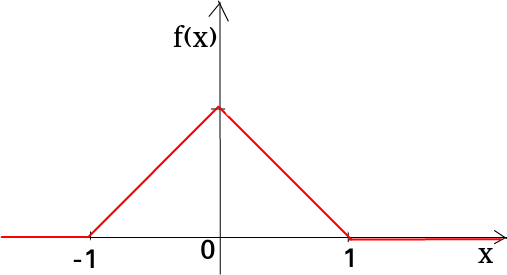
\includegraphics[width=.4\textwidth]{./pictures/16_15.png}
  \caption{График функции $f \left( x \right) $}
  \label{fig:1615}
\end{figure}

Тогда
$$Mf \left( \xi_n - \xi \right) =
\frac{1}{4} \left( 0 + 0 \right) + \frac{1}{2} \cdot 1 =
\frac{1}{2}.$$

При этом $Mf \left( 0 \right) = f \left( 0 \right) = 1$, но
$$ \frac{1}{2} \not \to 1, \,
n \rightarrow \infty.$$
Из этого следует, что $ \xi_n - \xi \not \Rightarrow 0, \, n \rightarrow \infty $.

\subsubsection*{16.17}

\textit{Задание.} Вычислить пределы:
\begin{enumerate}[label=\alph*)]
\item $ \lim \limits_{n \to \infty } \left( \frac{2}{ \pi } \right)^n
\idotsint \limits_{ \left[ 0, \infty \right]^n}
\sin \left( \frac{x_1 + x_2 + \dotsc + x_n}{n} \right)
e^{- \frac{2}{ \pi } \left( x_1 + x_2 + \dotsc + x_n \right) }
dx_1 dx_2 \dotsc dx_n$;
\item $ \lim \limits_{n \to \infty } \left( \frac{1}{ \sqrt{2 \pi }} \right)^n
\idotsint \limits_{ \mathbb{R}^n} \cos^{2m}
\left( \pi \cdot \frac{x_1 + x_2 + \dotsc + x_n}{n} \right) \times \\
\times e^{- \frac{ \left( x_1 - 1 \right)^2 + \dotsc + \left( x_n - 1 \right)^2}{2}}
dx_1 dx_2 \dotsc dx_n, \,
m \in \mathbb{N}$.
\end{enumerate}

\textit{Решение.}
\begin{enumerate}[label=\alph*)]
\item Запишем экспоненты в виде произведения
\begin{equation*}
\begin{split}
\lim \limits_{n \to \infty } \left( \frac{2}{ \pi } \right)^n
\idotsint \limits_{ \left[ 0, \infty \right]^n}
\sin \left( \frac{x_1 + x_2 + \dotsc + x_n}{n} \right) \times \\
\times e^{- \frac{2}{ \pi } \left( x_1 + x_2 + \dotsc + x_n \right) }
dx_1 dx_2 \dotsc dx_n = \\
= \lim \limits_{n \to \infty } \idotsint \limits_{ \left[ 0, \infty \right]^n}
\sin \left( \frac{x_1 + x_2 + \dotsc + x_n}{n} \right) \cdot
\frac{2}{ \pi } \cdot e^{- \frac{2}{ \pi } \cdot x_1} \times \\
\times \frac{2}{ \pi } \cdot e^{- \frac{2}{ \pi } \cdot x_2} \cdot \dotsc \cdot
\frac{2}{ \pi } \cdot e^{- \frac{2}{ \pi } \cdot x_n} dx_1 dx_2 \dotsc dx_n = \\
= \lim \limits_{n \to \infty } M \sin \left( \frac{ \xi_1 + \xi_2 + \dotsc + \xi_n}{n} \right), \,
\xi_n \sim Exp \left( \frac{2}{ \pi } \right)
\end{split}
\end{equation*}
--- независимые одинаково распределённые случайные величины.

Их математическое ожидание равно
$$M \xi_1 =
\frac{1}{ \frac{2}{ \pi }} =
\frac{ \pi }{2}.$$
По закону больших чисел
$$ \frac{ \xi_1 + \xi_2 + \dotsc + \xi_n}{n} \overset{P}{ \rightarrow } \frac{ \pi }{2}.$$

Тогда искомый предел равен
$$M \sin \left( \frac{ \xi_1 + \xi_2 + \dotsc + \xi_n}{n} \right) \to M \sin \frac{ \pi }{2} =
M1 = 1, \,
n \to \infty;$$
\item запишем экспоненты в виде произведения
\begin{equation*}
\begin{split}
\lim \limits_{n \to \infty } \left( \frac{1}{ \sqrt{2 \pi }} \right)^n
\idotsint \limits_{ \mathbb{R}^n} \cos^{2m}
\left( \pi \cdot \frac{x_1 + x_2 + \dotsc + x_n}{n} \right) \times \\
\times e^{- \frac{ \left( x_1 - 1 \right)^2 + \dotsc + \left( x_n - 1 \right)^2}{2}}
dx_1 dx_2 \dotsc dx_n = \\
= \lim \limits_{n \to \infty } \idotsint \limits_{ \mathbb{R}^n} \cos^{2m}
\left( \pi \cdot \frac{x_1 + x_2 + \dotsc + x_n}{n} \right) \cdot \frac{1}{ \sqrt{2 \pi }} \cdot
e^{- \frac{ \left( x_1 - 1 \right)^2}{2}} \times \\
\times \frac{1}{ \sqrt{2 \pi }} \cdot e^{- \frac{ \left( x_2 - 1 \right)^2}{2}} \cdot \dotsc \cdot
\frac{1}{ \sqrt{2 \pi }} \cdot
e^{- \frac{ \left( x_n - 1 \right)^2}{2}} dx_1 dx_2 \dotsc dx_n = \\
= \lim \limits_{n \to \infty } M \cos^{2m}
\left( \frac{ \xi_1 + \xi_2 + \dotsc + \xi_n}{2} \right), \,
\xi_n \sim N \left( 1, 1 \right)
\end{split}
\end{equation*}
--- независимые одинаково распределённые случайные величины.

Их математическое ожидание равно $M \xi_1 = 1$.

По закону больших чисел
$$ \frac{ \xi_1 + \xi_2 + \dotsc + \xi_n}{n} \overset{P}{ \rightarrow } M \xi_1 = 1.$$

Тогда исходный предел равен
$$M \cos^{2m} \left( \frac{ \xi_1 + \xi_2 + \dotsc + \xi_n}{n} \right) \to M \cos^{2m} \pi =
\cos^{2m} \pi = 1, \,
n \to \infty.$$
\end{enumerate}

\subsubsection*{16.18}

\textit{Задание.}
Пусть $ \left\{ \xi_n \right\}_{n \geq 1}$ --- последовательность независимых случайных величин,
каждая из которых имеет показательное распределение с параметром $ \lambda = 1$.
Докажите, что
$$ \left( \prod \limits_{k = 1}^n \xi_k \right)^{ \frac{1}{n}} \overset{P}{ \rightarrow } e^{-C}, \,
  n \to \infty.$$

\textit{Решение.} Сумму можно получить, прологарифмировав левую часть
$$ \ln \left( \prod \limits_{k = 1}^n \xi_k \right)^{ \frac{1}{n}} =
  \frac{1}{n} \left( \sum \limits_{k = 1}^n \ln \xi_k \right).$$

Так как $ \left\{ \ln \xi_n \right\}_{n \geq 1}$ ---
независимые одинаково распределённые случайные величины с конечным первым моментом, то
$$ \ln \left( \prod \limits_{k = 1}^n \xi_k \right)^{ \frac{1}{n}} \overset{P}{ \rightarrow }
  M \ln \xi_1 =
  \int \limits_0^{+ \infty } \lambda \ln x e^{- \lambda x} dx =
  \int \limits_0^{+ \infty } \ln x e^{- x} dx, \,
  n \to \infty.$$

Возьмём справа и слева экспоненту, поскольку экспонента --- непрерывная функция
$$ \left( \prod \limits_{k = 1}^n \xi_k \right)^{ \frac{1}{n}} \overset{P}{ \rightarrow }
  e^{ \int \limits_0^{+ \infty } \ln x e^{-x} dx} =
  e^{-C}, \,
  n \to \infty.$$
